\documentclass[11pt,english]{article}
\usepackage[a4paper,bindingoffset=0.1in,%
            left=0.5in,right=0.5in,top=0.5in,bottom=0.5in,%
            footskip=.25in]{geometry}
\usepackage[utf8]{inputenc}
\usepackage{graphicx}
\usepackage{hyperref}

\DeclareTextFontCommand{\textbackit}{\backitshape}
\begin{document}
\title{Speech Recognition Engine}
\author{Hrithik Raj (ES17BTECH11009)}

\sloppy
\maketitle
\setlength{\columnsep}{0.25in}
\twocolumn
\tableofcontents

\section{Introduction}
This consists details of speech recognition engine for a voice bot. 
The model used is based on concepts of Convolution, LSTM and Attention.

\section{Data Generation}
Used Audacity to generate your own voice samples.
\begin{enumerate}
    \item Set the sampling rate to 16 kHz
    \item Record 80 utterances of each command - forward, back, right, left, stop.
    \item Trim each utterance to one second.
    \item Save samples of each command in different folders as\\
        Dataset/forward\\
        Dataset/back\\
        Dataset/left\\
        Dataset/right\\
        Dataset/stop
\end{enumerate}
Use soundfile package to read the .wav. Other package like wavefile, librosa etc could also be used.\\
Store the loaded data as numpy file for ease and speed of access. Now, the data can be loaded from the numpy file if the experiment is repeated.

\section{Split dataset}
Split the dataset into train and test set with 80\% as train samples and 20\% as test samples.\\
Set a random seed for reproducing the split.

\section{Augment data}
Augment each audio sample by time shifting in 25000 length vectors filled with zeros. \\
Take steps of 500 to create 18 files per sample

\section{Feature Extraction}
MFCCs(Mel-Frequency Cepstral Coefficients) feature extraction is a leading approach for speech feature extraction.Normalizing the MFCCs over the frequency axis is found to reduce effect of noise.

Kapre is a python package that provides layers for audio processing that are compatible with keras and utilize GPU for faster processing. Kapre provides us with a layer basically.

\emph{Melspectrogram (padding = 'same', sr=16000, n\_mels = 39, n\_dft = 1024, power\_melgram = 2.0, return\_decibel\_melgram = True, trainable\_fb = False, trainable\_kernal = False, name = 'mel\_stft')}

\textbf{Arguments to the layer}

\textbf{padding} : Padding when convoluting

\textbf{sr} : Sampling rate of audio given

\textbf{n\_mels}: number of coefficients to return

\textbf{n\_dft}: width 

\textbf{power\_melgram} : exponent to raise log-mel-amplitudes before taking DCT. Using power 2 is shown to increase performance by reducing effect of noise

\textbf{return\_decibel\_melgram} : If to return log over values

\textbf{trainable\_fb} : If filter bank is trainable

\textbf{trainable\_kernel} : If the kernel is trainable

\section{Building Model}
\subsection{Concept}
\begin{enumerate}
    \item LSTMs(Long Short Term Memory Units) are a type of RNNs capable of learning order dependence in sequence prediction problems.
    \item Several research papers show that using Convolutional layers ahead of LSTM has shown to improve performance.
    \item BatchNormalization layers are added to improve convergence rate.
    \item Using Bidirectional LSTM is optimal when complete input is available. But this increases the runtime two-fold.
    \item Final output sequence of LSTM layer is used to calculate importance of units in LSTM using a FC layer.
    \item Then take the dot product of unit importance and output sequences of LSTM to get Attention scores of each time step.
    \item Take the dot product of Attention scores and the output sequences of LSTM to get attention vector.
    \item Add an additional FC Layer and then to output Layer with SoftMax Activation.
\end{enumerate}

\subsection{Parameters}
\begin{itemize}
    \item \textbf{sparse\_categorical\_crossentropy} is used as \textbf{Loss} because only output which should be 1 is given instead of One Hot Encoding.
    \item \textbf{sparse\_categorical\_accuracy} is used as performance \textbf{Metric} for the above reason.
    \item \textbf{Adam} is used as \textbf{Optimizer}. Adam is adaptive learning rate optimization algorithm. This is shown to achieve a faster convergence because of having all the features of other optimization algorithms.
    \item Batch size of 20 is used
\end{itemize}
Overall look of the architecture of the model is shown in Fig \ref{fig: Model} and the model diagram is shown in Fig \ref{fig: Model_diag}

\section{Training the Model}

\subsection{Back Propagation}
Back propagation is the algorithm used to calculate the gradient of loss w.r.t all the parameters in the neural network. Gradient of Loss w.r.t parameter is the direction in which the parameter should move such that decrease in loss will be maximum. It is the practice of fine-tuning the weights of a neural network based on the error rate (i.e. loss) obtained in the previous epoch (i.e. iteration). Proper tuning of the weights ensures lower error rates, making the model reliable by increasing its generalization.\\
Each layer and function is programmed to calculate the gradient of loss w.r.t it's trainable parameters and input given the input and gradient of loss w.r.t its output.\\
Gradient of loss w.r.t input of the current layer or function is back propagated as gradient of loss w.r.t output of previous layer or function. Hence, the name back propagation.

\subsection{Adam Optimizer}
Back propagation calculates the gradient of loss w.r.t each parameter. But an adaptive learning rate algorithm will be used to update the weights in a more calculated manner.\\
Adam is an optimization algorithm that can be used instead of the classical SGD procedure to update network weights iterative based in training data.Adam maintains few training parameters independently for each network parameter while SGD only has a single learning rate parameter for all the weights of the network. Adam is a combination of AdaGrad and RMSProp (Two other optimization algorithms).\\
RMSProp uses only Average first moment (running average of the gradient) while Adam also uses Average second moment (running average of the square of gradient ) in the learning rate calculation.\\
For each network parameter, Adam maintains 
\begin{itemize}
    \item \textbf{Alpha}
    Also referred to as the learning rate or step size. 
    Proportion of the update to be added to the weight.
    \item \textbf{Beta1}
    The exponential decay rate for the first moment estimates (e.g. 0.9).
    \item \textbf{Beta2}
    The exponential decay rate for the second-moment estimates (e.g. 0.999)
    \item \textbf{Epsilon}
    Is a very small number to prevent any division by zero in the implementation (e.g. 10E-8)
\end{itemize}


\begin{figure}[!ht]
\centering
\includegraphics[width=\columnwidth]{./Figs/Adam.eps}
\caption{ Adam algorithm}.
\label{fig: Adam}	
\end{figure}


\section{Testing}
\begin{enumerate}
    \item Augment the test set same as training set.
    \item Extract MFCCs same as above
    \item Test set is passed as validation set to fit method of model.
    \item The performance of model on test set is calculated after every epoch.
\end{enumerate}

\section{Visualize Attention}
\begin{enumerate}
    \item Now build a sub model from the trained model. Take same input layer but add ‘AttentionSoftmax’ layer as additional output layer.
    \item Pass MFCCs of test samples to predict method.
    \item Plot log of Attention Scores and corresponding input vector before taking MFCCs on different axes.
    \item By looking at Fig \ref{fig: Attention} and Fig \ref{fig: Sample}, We observe that Attention Scores are high on informative part.
    \begin{figure}[!ht]
    \centering
    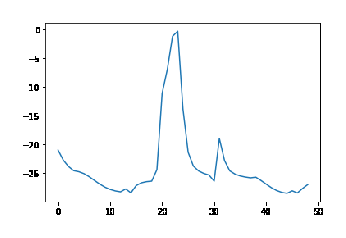
\includegraphics[width=\columnwidth]{./Figs/attention.eps}
    \caption{ log(Attention Scores)}.
    \label{fig: Attention}	
    \end{figure}
    \begin{figure}[!ht]
    \centering
    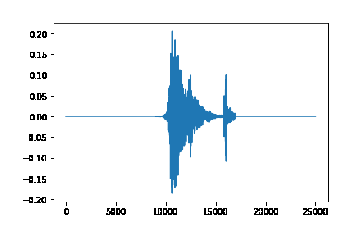
\includegraphics[width=\columnwidth]{./Figs/sample.eps}
    \caption{ Raw sample}.
    \label{fig: Sample}	
    \end{figure}
    
\end{enumerate}

\section{Observations}
\begin{itemize}
    \item Smaller batch size is prefferable
    \item Setting power\_melgram=2 of Melspectogram gave faster convergence.
\end{itemize}
\section{Functions}
Each block in the flowchart can be executed through a function mentioned below 
\begin{itemize}
    \item $data\_generation()$ : Generates the data
    \item $train\_test()$ : Splits the data into train and test and augments the data
    \item $feature\_ext()$: Extracts MFCC coefficients
    \item $model\_training()$: Trains model.
    \item $save\_model()$: Saves the model in h3 file
    \item $attention\_vis()$ : Checks Performance and visualize attention
    \item ColabNotebook.ipynb: Use this for experimental purpose
\end{itemize}

\begin{figure}[!ht]
\centering
\includegraphics[width=\columnwidth]{./Figs/flowchart.eps}
\caption{Flowchart}.
\label{fig: Flow}	
\end{figure}
%
\begin{figure}[!ht]
\centering
\includegraphics[width=\columnwidth]{./Figs/model_diag.eps}
\caption{ Model Diagram}.
\label{fig: Model_diag}	
\end{figure}

\onecolumn

\begin{figure}[!ht]
    \centering
    \includegraphics[width=\columnwidth]{./Figs/model.eps}
    \caption{Model Architecture}.
    \label{fig: Model}	
    \end{figure}

\end{document}
